\documentclass[a4paper, english, 12pt, reqno, draft]{amsart}

% ---------------------------------------------------------------------------

% Usepackages recommended in mcom-l-template.tex if needed.

\usepackage{amssymb}
% \usepackage{graphicx}
% \usepackage[cmtip,all]{xy}

% ---------------------------------------------------------------------------

% Usepackages inserted by authors.

\usepackage[english]{babel}
\usepackage[utf8]{inputenc}
\usepackage{tikz,tikzscale}
\tikzset{>=latex}
\usepackage{xcolor}
\usepackage{enumerate}
\usepackage{booktabs,multirow}
\usepackage{amsfonts}

%%%%%%%%%% Packages to help editing %%%%%%%%%%
\usepackage[notref,notcite]{showkeys} % Show labels.
\usepackage[mode=multiuser]{fixme} % Provide note, warning, error, fatal.
\FXRegisterAuthor{gk}{envgk}{GK}
\FXRegisterAuthor{ar}{envar}{AR}
\fxusetheme{color}

% ---------------------------------------------------------------------------

% Theorems in the AMS style.

\newtheorem{theorem}{Theorem}[section]
\newtheorem{lemma}[theorem]{Lemma}
\newtheorem{corollary}[theorem]{Corollary}

\theoremstyle{definition}
\newtheorem{definition}[theorem]{Definition}
\newtheorem{example}[theorem]{Example}
\newtheorem{exercise}[theorem]{Exercise}

\theoremstyle{remark}
\newtheorem{remark}[theorem]{Remark}

\numberwithin{equation}{section}

% ---------------------------------------------------------------------------

% Newcommands by the authors.

\newcommand{\graph}{\ensuremath{\mathcal G}}
\newcommand{\setEdge}{\ensuremath{\mathcal E}}
\newcommand{\setNode}{\ensuremath{\mathcal N}}
\newcommand{\setNodeDir}{\ensuremath{\setNode_\textup D}}
\newcommand{\setNodeNeu}{\ensuremath{\setNode_\textup N}}
\newcommand{\setNodeInt}{\ensuremath{\setNode_\textup I}}
\newcommand{\edge}{\ensuremath{E}}
\newcommand{\node}{\ensuremath{N}}

\newcommand{\Graph}{\ensuremath{\boldsymbol{\mathcal G}}}
\newcommand{\SetEdge}{\ensuremath{\boldsymbol{\mathcal E}}}
\newcommand{\SetNode}{\ensuremath{\boldsymbol{\mathcal N}}}
\newcommand{\SetNodeDir}{\ensuremath{\SetNode_\textup D}}
\newcommand{\SetNodeNeu}{\ensuremath{\SetNode_\textup N}}
\newcommand{\SetNodeInt}{\ensuremath{\SetNode_\textup I}}
\newcommand{\Edge}{{\ensuremath{\boldsymbol E}}}
\newcommand{\RefEdge}{{\ensuremath{\widehat{\boldsymbol e}}}}
\newcommand{\Node}{{\ensuremath{\boldsymbol N}}}

\newcommand{\locDim}{\ensuremath{\mathfrak d}}
\newcommand{\globDim}{\ensuremath{\mathfrak D}}

\newcommand{\Der}{\ensuremath{\textup d_\Edge}}
\newcommand{\Nabla}{\ensuremath{\nabla_\Edge}}
\newcommand{\Div}{\ensuremath{\Nabla\!\cdot\!}}
\newcommand{\tangent}{\ensuremath{{\boldsymbol T}}}
\newcommand{\Normal}{\ensuremath{\mathfrak n_\Edge}}
\newcommand{\NormalOuter}{\ensuremath{\mathfrak n^\perp_\Edge}}
\newcommand{\jump}[1]{{[\![ #1 ]\!]}}
\newcommand{\diffeo}{\ensuremath{\Phi}}
\newcommand{\tangentMapping}{\ensuremath{\Phi_{\tangent(x)}}}
\newcommand{\orthProj}{\ensuremath{\Pi_{\tangent(x)}}}

\newcommand{\IN}{\ensuremath{\mathbb N}}
\newcommand{\IR}{\ensuremath{\mathbb R}}

\newcommand{\elem}{\ensuremath{T}}
\newcommand{\mesh}{\ensuremath{\mathcal T}}
\newcommand{\meshIndex}{\ensuremath{\mathcal I}}
\newcommand{\faceSet}{\ensuremath{\mathcal F}}
\newcommand{\faceSetDir}{\ensuremath{\mathcal F^\textup D}}
\newcommand{\face}{\ensuremath{F}}
\newcommand{\skeletal}{\ensuremath{\Sigma}}
\newcommand{\skeletalSpace}{\ensuremath{M}}
\newcommand{\skeletalSpaceHDG}{\ensuremath{M}}
\newcommand{\contElementSpace}{\ensuremath{V^\textup c}}
\newcommand{\contThreeElementSpace}[1]{\ensuremath{V^\textup c_{#1,p+3}}}
\newcommand{\linElementSpace}{\ensuremath{\overline V^\textup c}}
\newcommand{\discElementSpace}{\ensuremath{V}}
\newcommand{\polynomials}{\ensuremath{\mathcal P}}
\newcommand{\level}{\ensuremath{\ell}}
\newcommand{\iterMgOuter}{i}%\ensuremath{\nu}}
\newcommand{\iterMgInner}{m}%\ensuremath{\eta}}

\newcommand{\discLaplacian}{\ensuremath{A}}
\newcommand{\extensionOp}{\ensuremath{\mathcal U^\textup c}}
\newcommand{\averagingOp}{\ensuremath{I^\textup{avg}}}
\newcommand{\restrictionOp}{\ensuremath{I^\textup{res}}}
\newcommand{\traceOp}{\ensuremath{\gamma_0}}
\newcommand{\injectionOp}{\ensuremath{I}}
\newcommand{\projectionOp}{\ensuremath{P}}
\newcommand{\projectionOrthogonalOP}{\ensuremath{\Pi}}
\newcommand{\projectionLinOp}{\ensuremath{\overline P}}
\newcommand{\skeletalProj}{\ensuremath{\Pi^\partial}}
\newcommand{\contLinProj}{\ensuremath{\overline \Pi^\textup c}}
\newcommand{\discProj}{\ensuremath{\Pi^\textup d}}
\newcommand{\liftingOp}{\ensuremath{S}}

\renewcommand{\vec}[1]{\ensuremath{\boldsymbol{#1}}}
\newcommand{\Nu}{\ensuremath{\vec \nu}}
\newcommand{\dx}{\ensuremath{\, \textup d x}}
\newcommand{\ds}{\ensuremath{\, \textup d \sigma}}
\newcommand{\localU}{\ensuremath{\mathcal U}}
\newcommand{\localQ}{\ensuremath{\vec{\mathcal Q}}}
\newcommand{\penaltyParam}{\ensuremath{\eta}}

\newcommand{\tildelambda}{\tilde\lambda}
\newcommand{\ureconstructed}{\overline{u}}
\newcommand{\projectionBramble}{\ensuremath{\bar B}}
\newcommand{\indexDOF}{\ensuremath{i}}
\newcommand{\IndexDOF}{\ensuremath{\mathcal I}}

\newcommand{\llangle}{\ensuremath{\langle \! \langle}}
\newcommand{\rrangle}{\ensuremath{\rangle \! \rangle}}
\newcommand{\nnorm}{\ensuremath{\vert \! \vert \! \vert}}

% ---------------------------------------------------------------------------

% Make paragraph heading being small capitals!

\makeatletter
\def\paragraph{\@startsection{paragraph}{4}%
  \z@\z@{-\fontdimen2\font}%
  {\normalfont\scshape}}
\makeatother

% ---------------------------------------------------------------------------

% Usepackage hyperref is the last to be added!

\usepackage[colorlinks = true, linkcolor = blue, citecolor = blue, urlcolor = blue]{hyperref}

% ---------------------------------------------------------------------------

% Document head as described in the template.

\begin{document}

\title[H\MakeLowercase{yper}HDG --- HDG on hypergraphs]{H\MakeLowercase{yper}HDG --- Hybrid disontinuous Galerkin methods for PDEs on hypergraphs} 

\author{Andreas Rupp}
\address{Interdisciplinary Center for Scientific Computing (IWR), Heidelberg University, Mathematikon, Im Neuenheimer Feld 205, 69120 Heidelberg, Germany}
% \curraddr{}
\email{andreas.rupp@fau.de, andreas.rupp@uni-heidelberg.de}
\thanks{This work is supported by the Deutsche Forschungsgemeinschaft (DFG, German Research Foundation) under Germany's Excellence Strategy EXC 2181/1 - 390900948 (the Heidelberg STRUCTURES Excellence Cluster).}

\author{Guido Kanschat}
\address{Interdisciplinary Center for Scientific Computing (IWR) and Mathematics Center Heidelberg (MATCH), Heidelberg University, Mathematikon, Im Neuenheimer Feld 205, 69120 Heidelberg, Germany}
% \curraddr{}
\email{kanschat@uni-heidelberg.de}
% \thanks{}

\subjclass[2010]{\textcolor{red}{TODO}}

\date{\today}

% \dedicatory{}

\begin{abstract}
 \textcolor{red}{\textsc{Todo!}} 
 \\[1ex] \noindent \textsc{Keywords.}
 \textcolor{red}{TODO!}
\end{abstract}
% 
\maketitle
% 
\section{Introduction}
% 
% ---------------------------------------------------------------------
\section{Hypergraphs}\label{SEC:hypergraph}
% ---------------------------------------------------------------------
% 
HyperHDG is a simumlation software to perform numerical experiments on so called hypergraphs. To this end, it is useful to discuss the composition of hypergraphs in some detail. At first, every hypergraph is defined as topological hypergraph, cf. Section. \ref{SEC:hypergraph_topology}. Additionally, a hypergraph may be equipped with a geometry, as illuminated in Section \ref{SEC:hypergraph_geometry}. 
% 
\subsection{Topologic aspects of hypergraphs}\label{SEC:hypergraph_topology}
% 
In the whole manuscript, we consider a \emph{hypergraph} $\graph = (\setNode,\setEdge)$ consisting of a finite set of \emph{hypernodes} $\setNode = \{\node_1, \node_2, \ldots \}$ and a set of \emph{hyperedges} $\setEdge = \{\edge_1, \edge_2, \ldots \}$. All hyperedges $\edge \in \setEdge$ can be interpreted as connecting several nodes and, thus, can be written as $\edge \subset \setNode$.

Thus, the topology of a hypergraph $\graph$ is a pair consisting of a set of hyperedges $\setEdge$ and a set of hypernodes $\setNode$. Each hyperedge $\edge \in \setEdge$ is connected to other hyperedges via the set of its adjacent hypernodes. Note that this is exactly the inverted interpretation as compared to the aforementioned definition of a hypergraph, where nodes are interpreted as connected via edges.

\paragraph{Cubic and simplicial hypergraphs, and local dimension $\locDim$}
% 
We will define partial differential equations (PDEs) on hypergraphs. To do so, it helps---but is not necessary---to have an adequate graphical representation of hyperedges. For example, one might try to represent all $\edge \in \setEdge$ as (relatively) open unit hypercubes of dimension $\locDim \in \IN$. A hypergraph, of which all hypereges $\edge = \{ \node_1, \node_2, \ldots, \node_{2\locDim} \}$ consist of exactly $2\locDim$ hypernodes, allows for such a representation of all hyperedges. The hypernodes may then be interpreted as the \emph{faces} (not the vertices) of the hypercubes/hyperedges and the hypergraph is denoted \emph{cubic} of \emph{local dimension} $\locDim$. In this representation, also the hypernodes are supposed to be (relatively) open sets.

Analogously, a hypergraph of which all hyperedges consist of $\locDim+1$ is called simplicial of local dimension $\locDim$.

\paragraph{Cubic/simplicial (topological) embeddings of hypergraphs to global dimension $\globDim$}
% 
If one wants to represent the whole hypergraph at once (instead of only single hyperedges), an embeddind to an $\globDim$ dimensional space is needed. To allow for an easy notation, we denote by $\Edge \in \SetEdge$ the representation of $\edge \in \setEdge$ as (relatively) open hypercube/simplex, by $\node \in \setNode$ the representation of a hypernode $\Node \in \SetNode$ as (relatively) open face, and set $\Graph = (\SetNode, \SetEdge)$. A cubic/simplicial hypergraph can be topologically embedded into $\IR^\globDim$ if
% 
\begin{enumerate}
 \item there is a way to assemble all unit hypercubes/simplices (representing the hyperedges) such that for two hyperedges $\edge^+ \neq \edge^-$ and two hypernodes $\node^- \neq \node^+$, we have $\Edge^- \cap \Edge^+ = \emptyset$ and $\Node^- \cap \Node^+ = \emptyset$.
 \item in the aforementioned assembly for all $\node \in \setNode$ and $\edge \in \setEdge$: We have $\Node \cap \Edge \neq \emptyset$ if, and only if, $\node \in \edge$.
\end{enumerate}
% 
\paragraph{Examples for cubic hypergraphs}
% 
According to this definition, every graph is both a cubic and a simplicial hypergraph. An illustration which can be interpreted as several hypergraphs---all embedded to $\globDim = 3$---can be found in Figure \ref{FIG:hyG_topo}:
% 
\begin{itemize}
 \item Cubic or simplicial hypergraph of $\locDim = 1$ consisting of twelve hypernodes (vertices) and  twenty hyperedges (lines).
 \item Cubic hypergraph of $\locDim = 2$ consisting of twenty hypernodes (lines) and eleven hyperedges (squares).
 \item Cubic hypergraph of $\locDim = 3$ consisting of two eleven hypernodes (squares) and two hyperedges (cubes).
\end{itemize}
% 
\begin{figure}[ht]
 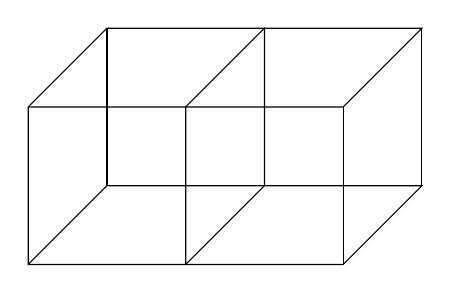
\begin{tikzpicture}
  \draw (0,0) -- (2,0) -- (4,0) -- (5,1) -- (3,1) -- (1,1) -- (0,0) -- (0,2) -- (2,2) -- (4,2) -- (5,3) -- (3,3) -- (1,3) -- (0,2);
  \draw (2,0) -- (3,1) -- (3,3) -- (2,2) -- (2,0);
  \draw (1,1) -- (1,3);
  \draw (4,0) -- (4,2);
  \draw (5,1) -- (5,3);
 \end{tikzpicture}
 \caption{Illustration that can be interpreted as several types of hypergraph topologies.}\label{FIG:hyG_topo}
\end{figure}
% 
\subsection{Geometrical aspects of hypergraphs}\label{SEC:hypergraph_geometry}
% 
Figure \ref{FIG:hyG_topo} already indicates that hypergraphs, especially those with embeddings might be equipped with geometrical information. This specific example indicates that all lines, squares, cubes are of unit size. However, the hypergraph might also have geometrical information that says it looks like in Figure \ref{FIG:hyG_geom}, where the first picture is valid for all $\locDim$ and the second one is only valid for $\locDim = 3$. Note that, all sufaces may also be curved, but we restrict to straight representations, here.
% 
\begin{figure}[ht]
 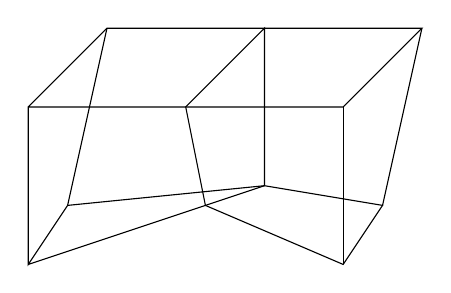
\begin{tikzpicture}
  \draw (0,0) -- (2.25,0.75) -- (4,0) -- (4.5,0.75) -- (3,1) -- (0.5,0.75) -- (0,0) -- (0,2) -- (2,2) -- (4,2) -- (5,3) -- (3,3) -- (1,3) -- (0,2);
  \draw (2.25,0.75) -- (3,1) -- (3,3) -- (2,2) -- (2.25,0.75);
  \draw (0.5,0.75) -- (1,3);
  \draw (4,0) -- (4,2);
  \draw (4.5,0.75) -- (5,3);
 \end{tikzpicture}
 \quad
  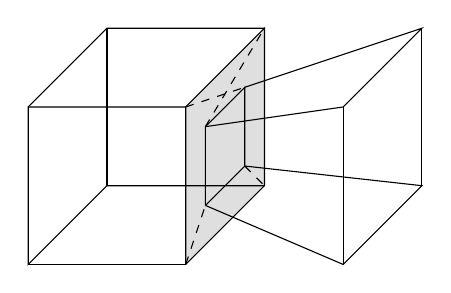
\begin{tikzpicture}
  \path[fill=gray!25] (2,0) -- (3,1) -- (3,3) -- (2,2) -- (2,0);
  \draw (0,0) -- (2,0);
  \draw[dashed] (2,0) -- (2.25,0.75);
  \draw (2.25,0.75)  -- (4,0) -- (5,1) -- (2.75,1.25);
  \draw[dashed] (2.75,1.25) -- (3,1);
  \draw (3,1) -- (1,1) -- (0,0) -- (0,2) -- (2,2);
  \draw (2.25,1.75) -- (4,2) -- (5,3) -- (2.75,2.25); 
  \draw (3,3) -- (1,3) -- (0,2);
  \draw[dashed] (2,2) -- (2.75,2.25);
  \draw[dashed] (2.25,1.75) -- (3,3);
  \draw (2,0) -- (3,1) -- (3,3) -- (2,2) -- (2,0);
  \draw (2.25,0.75) -- (2.75,1.25) -- (2.75,2.25) -- (2.25,1.75) -- (2.25,0.75);
  \draw (1,1) -- (1,3);
  \draw (4,0) -- (4,2);
  \draw (5,1) -- (5,3);
 \end{tikzpicture}
 \caption{Two possible geometrical representation of the hypergraph in Figure \ref{FIG:hyG_topo}. The second one is only valid for $\locDim = 3$---the gray hypernode has different geometrical representations for the two adjacent hyperedges.}\label{FIG:hyG_geom}
\end{figure}

This motivates the following observation: A hypergraph can, beyond its topological information, carry geometrical information. That is, for all hyperedges, there is a geometry prescribed.

This can lead to the case that for one hypernode, different geometries are prescribed as illustrated gray in the right picture of Figure \ref{FIG:hyG_geom}. The hypernode can also be disorted as illustrated by the dashed lines indicating that the two top vertices have to interchange when reinterpreting the node as face of the one or the other hyperedge. This could not be easily illustrated in the picture if the right version of the hypernode was not smaller than the left version. Thus, the hypernode would look as if no reinterpretation is necessary, although in fact, it is.

\paragraph{Embedded hypergraphs}
% 
If the hypergraph can be topologically embedded to dimension $\globDim$ and carries geometrical information for the hyperedges, such that for all hypernodes, there is a unique geometrical description---excluding that the hypernode is disorted or has different shapes for different hyperedges, then the hypergraph can be \emph{topological and geometrical embedded} (for short, just \emph{embedded}) into $\IR^\globDim$. For the representation of the embeddded hypergraph, we also use the notation with the bold symbols.

\paragraph{Smoothness assumptions}
% 
We assume that all hyperedges $\IR^\globDim \supset \Edge \in \SetEdge$ allow for a $C^\infty$ diffeomorphism
% 
\begin{equation*}
 \diffeo \colon \; \IR^\locDim \supset \RefEdge ~\mapsto~ \Edge \subset \IR^\globDim,
\end{equation*}
% 
where the reference element $\RefEdge$ is either a unit simplex of a unit hypercube.

Thus, the $\Edge\in \setEdge$ are \emph{Riemannian manifolds}, i.e., they are real, smooth manifolds, and for all $x \in \Edge$, they are equipped with an inner product $(\cdot,\cdot)_{\tangent(x)}$ with respect to the tangent space $\tangent(x)[\Edge] \subset \IR^\globDim$ of the manifold $\Edge$ evaluated at point $x$. If no confusion is possible, the expression $[\Edge]$ is dropped. We set the inner product as standard Euclidean scalar product
% 
\begin{equation*}
 (a,b)_{\tangent(x)} = (a,b)_{\IR^\globDim} =: (a,b) \qquad \text{ for all } a,b \in \tangent(x) \text{ and } x \in \Edge
\end{equation*}
% 
and define $\| x \|^2 := (x,x)$ for $x \in \IR^\globDim$.

\paragraph{Linear hypergraphs}
% 
A cubic/simplicial hypergraph is called \emph{linear} if all hyperedges $\SetEdge \ni \Edge \subset \IR^\globDim$ can be represented as image of an affine-linear mapping of a (reference) unit hypercube/simplex $\RefEdge \subset \IR^\locDim$. This implies that all faces are straight and that the transformation is square if and only is $\locDim = \globDim$.
% ---------------------------------------------------------------------
\section{Model equation and interpretation}\label{SEC:model_eq}
% ---------------------------------------------------------------------
% 
Here, we formulate the standard diffusion equation in mixed form defined on a hypergraph $\graph$ that for the moment is assumed to allow an embedding $\Graph$. The differential operators will be rigorously defined in Section \ref{SEC:diff_op}. Thus, for all $\Edge \in \SetEdge$ we approximate solutions $(u, \vec q)$ of
% 
\begin{subequations}\label{EQ:diffusion_mixed}
\begin{align}
 \Div \vec q & = f && \text{ in } \Edge,\label{EQ:div_is_f}\\
 \tfrac{1}{d} \vec q + \Nabla u & = 0 && \text{ in } \Edge.\label{EQ:primal_dual}
\end{align}
% 
for a given functions $d \ge d_0 > 0$ and $f$. Here, $u$ may be considered as concentration and $\vec q$ as flux of a chemical species diffusing on the hypersurface $\Edge$.

Additionally, we assume that there is a non-empty set $\setNodeDir \subset \setNode$ of Dirichlet hypernodes, a possibly empty set $\setNodeNeu \subset \setNode\setminus \setNodeDir$ of Neumann hypernodes, and the remainder set $\setNodeInt = \setNode \setminus (\setNodeDir \cup \setNodeNeu)$ of interior hypernodes. The following ideas motivate three different types of closing conditions:
% 
\begin{itemize}
 \item On hypernodes of Dirichlet type, the value of function $u$ is prescribed by function $u_\text D$.
 \item On hypernodes of Neumann type, outflow of the whole system/hypergraph with rate $g_\textup N$ is prescribed. The outflow of chemical species with respect to a hyperedge is defined via $\vec q \cdot \Normal$. Here, $\Normal$ is the outward unit normal with respect to the hyperedge, cf. Section \ref{SEC:normals}. Thus the sum of outflows of all hyperedges adjacent to the Neumann node should be equal to $g_\textup N$.
 \item Interior hypernodes are Neumann hypernodes with $g_\textup N \equiv 0$ describing conservation of the chemical species.
\end{itemize}
% 
For PDEs on manifolds or the full space, the sum of outflows of all hyperedges adjacent to a hypernode consists of either one (at the boundary) or two summands and typically is represented by the notion of a \emph{jump} $\jump{\vec q}$, which can be generalized to
% 
\begin{equation*}
 \jump{\vec q} = \sum^{\edge \in \setEdge}_{\edge \ni \node} \vec q_\Edge \cdot \Normal \quad \text{ with } \quad \vec q_\Edge = \vec q|_\Edge,
\end{equation*}
% 
which turns the vector function $\vec q$ to a scalar and is defined for all hyppernodes. Using this generalization, the closing conditions can be formulated into the following equations:
% 
\begin{align}
 u & = u_\textup D && \text{ on } \Node \in \SetNodeDir,\label{EQ:dir_cond}\\
 \jump{\vec q} & = g_\textup N && \text{ on } \Node \in \SetNodeNeu,\label{EQ:neu_cond}\\
 \jump{\vec q} & = g_\textup N && \text{ on } \Node \in \SetNodeNeu.\label{EQ:int_cond}
\end{align}
\end{subequations}
% 
Thus, \eqref{EQ:diffusion_mixed} is a direct generalization of the standard diffusion equation in the whole space---even with the same notation---if we manage to find proper direct generalizations of normals and differential operators.
% 
\subsection{The notion of normals}\label{SEC:normals}
% 
In the following, we will define different notions of normals with respect to a hyperedge $\Edge \in \SetEdge$. The simplest type of normal is the outer normal which is defined via
% 
\begin{equation*}
 \|\NormalOuter(x)\| = 1 \qquad \text{ and } \qquad (\NormalOuter(x), v) = 0 \quad \text{ for all } v \in \tangent(x).
\end{equation*}
% 
The second condition can be abbreviated to $\NormalOuter(x) \perp \tangent(x)$.

For each point $x \in \Edge$ there either exist no ($\locDim = \globDim$), two ($\locDim = \globDim - 1$) or infinitely many outer normals. Additionally, for $x \in \partial \Edge$, we define the inner normal $\Normal$ as unique, outward pointing vector with
%
\begin{equation*}
 \| \Normal \| = 1, \qquad \Normal \in \tangent(x), \qquad \Normal \perp \tangent(x) [\partial \Edge]
\end{equation*}

% 
\subsection{Differential operators on hyperedges}\label{SEC:diff_op}
% 
Consider the smooth function $f: \Edge \to \IR$. Its \emph{directional derivative} in $x \in \Edge$
% 
\begin{equation}\label{EQ:direc_der}
 [\Der f(x)](v) ~:=~ \frac{\textup d}{\textup d \tau} (f \circ \gamma)(\tau)|_{\tau = 0}
\end{equation}
% 
for any smooth curve $\gamma: (-1,1) \to \Edge$ with $\gamma(0) = x$ and $\gamma'(0) = v$. Here, $v$ is called the \emph{direction}.

Accordingly, the \emph{derivative} is defined as
% 
\begin{equation*}
 \Der f(x) \colon \tangent(x) \to \IR, \qquad \text{ \eqref{EQ:direc_der} holds for all $v \in \tangent(x)$.}
\end{equation*}
% 
Thus, $\Der f(x) \in \tangent^\star(x)$ which is the dual space of $\tangent x$ and there is a well-defined mapping $\Der f \colon \Edge \to \tangent^\star(x)$. According to Riesz representation theorem, there is a unique \emph{gradient} $\Nabla f \colon \Edge \to \tangent(x)$ with
% 
\begin{equation*}
 (\Nabla f(x), v) = [\Der f(x)](v) \qquad \forall x \in \Edge, \forall v \in \tangent(x).
\end{equation*}
% 
In terms of muscial isomorphisms, that is
% 
\begin{equation*}
 \Nabla f = (\Der f)^\sharp \qquad \text{ and } \qquad \Der f = (\Nabla f)^\flat.
\end{equation*}

The definition of the \emph{divergence} of a smooth vector function $\vec f \colon E \to \IR^\locDim$ can be done using an orthonormal basis $\mathcal B$ of $\tangent(x)$---which contains $\locDim$ elements---and setting
% 
\begin{equation*}
 \Div \vec f: \Edge \to \IR, \qquad [\Div \vec f](x) = \sum_{b \in \mathcal B} [\Der (f, b)_{\IR^\locDim} (x)](b).
\end{equation*}
% ---------------------------------------------------------------------
\section{HDG methods on hypergraphs}
% ---------------------------------------------------------------------
%
Starting out from a subdivision $\graph = (\setEdge, \setNode)$.

By $\faceSet$ we denote the set of faces of $\mesh_\level$.
The subset of faces on the boundary is
\begin{gather}
  \faceSetDir_\level := \{\face \in \faceSet_\level : \face \subset \partial \Omega \}.
\end{gather}
Moreover, we define
$\faceSet^\elem_\level := \{ \face \in \faceSet_\level : \face \subset
\partial \elem \}$ as the set of faces of a cell $\elem\in\mesh_\level$.  On the set of faces, we define the space $L^2(\faceSet_\ell)$ as the space of
square integrable functions with the inner product
\begin{gather}
  \llangle \lambda, \mu \rrangle_\level = \sum_{\elem \in \mesh_\level} \int_{\partial \elem} \lambda\mu\ds,
\end{gather}
and its induced norm
$\nnorm \mu \nnorm^2_\level = \llangle \mu, \mu
\rrangle_\level$. Note that interior faces appear twice in this definition such that expressions like $\llangle u, \mu \rrangle_\level$ with possibly discontinuous $u|_{\elem} \in H^1(\elem)$ for all $\elem \in \mesh_\level$ and $\mu \in L^2(\faceSet)$ are defined without further ado. Additionally, we define an inner product
commensurate with the $L^2$-inner product in the bulk domain, namely
\begin{gather}
  \langle \lambda, \mu \rangle_\level
  = \sum_{\elem \in \mesh_\level} \frac{|\elem|}{|\partial \elem|}
  \int_{\partial \elem} \lambda \mu \ds \cong \sum_{\face \in \faceSet_\level} h_\face
  \int_{\face} \lambda \mu \ds.
\end{gather}
Its induced norm is $ \| \mu \|^2_\level = \langle \mu, \mu \rangle_\level$.

Let $p\ge 1$ and $\polynomials_p$ be the space of (multivariate)
polynomials of degree up to $p$. Then, we define the space of piecewise
polynomials on the skeleton by
\begin{gather}
  \label{EQ:skeletal_space}
  \skeletalSpace_\level := \left\{ \lambda \in L^2(\faceSet_\level) \;\middle|\;
    \begin{array}{r@{\,}c@{\,}ll}
  \lambda_{|\face} &\in& \polynomials_p & \forall \face \in \faceSet_\level\\
  \lambda_{|\face} &=& 0 & \forall \face \in \faceSetDir_\level    
    \end{array}
  \right\}.
\end{gather}

The HDG method involves a local solver on each mesh cell
$\elem \in \mesh_\level$, producing cellwise approximations $u_\elem \in V_\elem$
and and $\vec q_\elem\in \vec W_\elem$ of the functions $u$ and $\vec q$ in
equation~\eqref{EQ:diffusion_mixed}, respectively. We choose
$V_\elem = \polynomials_p$. Then, choosing
$\vec W_\elem = \polynomials_p^d$ yields the so called hybridizable local discontinuous Galerkin (LDG-H) scheme. Our current analysis is in fact limited to this case and other choices require a modification of Lemma~\ref{LEM:u_q_bound}. We will also use the concatenations of the spaces $V_\elem$
and $\vec W_\elem$, respectively, as a function space on $\Omega$, namely
\begin{gather}
  \label{EQ:dg_spaces}
  \begin{aligned}
    \discElementSpace_\level
    &:=\bigl\{ v \in L^2(\Omega)
    & \big|\;v_{|\elem} &\in V_\elem,
    &\forall \elem &\in \mesh_\level \bigr\},\\
    \vec W_\level
    &:=\bigl\{ \vec q \in L^2(\Omega;\mathbb R^d)
    & \big|\;\vec q_{|\elem} &\in \vec W_\elem,
    &\forall \elem &\in \mesh_\level \bigr\}.    
  \end{aligned}
\end{gather}
%\begin{alignat}2
% \end{alignat}
\newpage
% 
\bibliographystyle{alpha}
\bibliography{HyperHDG}
% 
\end{document}
